Upon completion of the vehicle body construction and mounting the electronic components, significant
weight balance issues began to present themselves. Since a hovercraft is practically floating on a thin
layer of air, it is highly sensitive to weight imbalance. This imbalance caused
the hovercraft to stray (yaw\footnote{In 3 dimensions, the angle of the vertical axis.}), making it difficult to control.
Presented with such a situation, a PID controller could potentially correct the
imbalance issues by having the hovercraft automatically compensate to the yaw
produced by the imbalance.

\subsection{PID Controller Primer}
The acronym PID stands for Proportional, Integral, Derivative. These three
terms are used to define the behavior of the controller. Each contributes to the final output of the controller, and different weights can be
assigned to different terms. The weight selection process (tuning) is not an
easy task. In a nutshell, a PID controller can output corrective actions based
on the difference (error) between a set point (SP), the desired value and a
measured process variable (PV), the instantaneous value. A PID controller is a
feedback control loop wherein the output of the controller is treated as an
input of the same controller. The feedback allows the controller to
intelligently adjust its output according to the error. 

\begin{figure}[ht]
  \begin{center}
    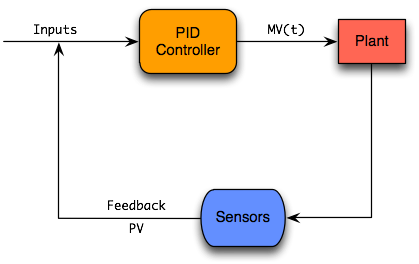
\includegraphics[width=85mm]{imageSources/pidcontroller.png}
  \end{center}
  \caption{A simple PID controller} 
  \label{pidController}
\end{figure}

The object being controlled by the PID controller is usually referred as the
plant, as shown in Figure \ref{pidController}. Depending on the system, a plant can be a
motor, servo, actuator, etc. The plant is constantly monitored by 
sensors in order for the PID controller to adjust its output based on the error.

\subsection{PID Terms}
There are three terms that determine the behavior of the
PID controller. The calculated output or Manipulated Variable (MV) of the PID
controller is the summation of all three terms. The formula can be written as:
\begin{displaymath}
MV(t) = K_pe(t) + K_d\frac{de}{dt}(t) + K_i\int\limits_{0}^{t} e\, dt
\end{displaymath}
where $K_p$, $K_d$, and $K_i$ are the weight constants or the tuning parameters,
and e is the error calculated by subtracting the set point(SP) by the process
variable(PV) or SP - PV.

\subsubsection{Proportional Term}
The proportional term in the PID controller corresponds to how fast the
controller reacts to error. Depending on the parameter $K_p$, the magnitude of
the proportional term will either amplify or diminish in the presence of error.
However, an improper choice for $K_p$ can lead to an unstable system.  When the value of $K_p$ is too large or too small, the output , $MV(t)$, of the controller will overshoot and take a long time to reach the set
point(SP), the desired value. 

\subsubsection{Derivative Term}
The derivative term determines the rate of which $e(t)$ is changing with
respect of time. The rate can be calculated by taking the first derivative of
the error over time. For example, if $K_d$ is set too high, meaning the
controller's output will converge to the set point very quickly, but it will run
into the problem of overshooting. By adding the derivative term, the output of
the controller can be slowed down as it gets closer and closer to the set point.
In other words, the derivative term can minimize overshoot and slightly improve
the converge time. One problem with the derivative term is that it is very
sensitive to noise. For instance, if the error rate is changing constantly, but
the sampling rate of the sensors is not constant, then this noise will
inadvertently propagate to the output of the controller and possibly amplify by
$K_d$. 

\subsubsection{Integral Term}
Both the proportional term and derivative term deal with the convergent
time(rise time) and the problem of overshooting. However, they don't take into
account of whether the output of the plant is actually equal to the set point
(steady state), and how to minimize the steady state error. Integral term takes
into account of the accumulated errors within a period of time. It ensures that
the output of the plant has reached the set point and it will stay at the set
point until a new set point is defined. Moreover, a small steady state error may
not be noticeable by the proportional term until the error becomes very large.
Hence, the integral can detect slight variation between the set point and output
and make proper adjustments accordingly. 

\subsection{Tuning}
The values for $K_p$, $K_d$, and $K_i$ can greatly affect the performance of the
PID controller. Moreover, the values for those constants must be tuned according
to the system that employs the PID controller. There isn't a set of values that
will work for multiple systems.  A decent reference on tuning a PID system is
\cite{Skogestad2003291}.  Although the paper is primarily concerned with
chemical systems the principles remain the same.  

\subsection{PID Controller and Hovercraft}
The PID controller logic will be implemented in AT90USB. Since our design of the
hovercraft uses two motors for thrust as well as for turning, the plants will be
the two motors. The sensors will be described below. The following diagram
describes how the plants, PID controller, and sensors interact. The connections
connecting the two motors and the sensors are dotted because the sensors are not
directly monitoring the RPM of the motors. The sensors are constantly monitoring
the heading, yaw rate, and motions. 

\begin{figure}[ht]
  \begin{center}
    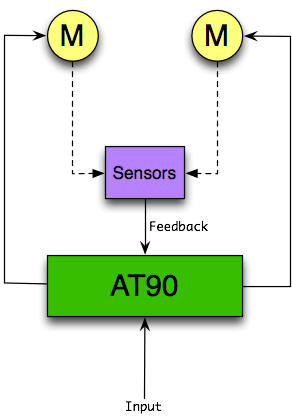
\includegraphics[width=85mm]{imageSources/pidhovercraft.png}
  \end{center}
  \caption{Hovercraft PID controller} 
  \label{pidController}
\end{figure}

Sensors are necessary to keep the hovercraft heading straight and steady and
essential to the PID controller as they provide feedback information. In order
to navigate the environment without running into obstacles, hovercraft will use
sonars for ranging. A magnetometer to detect the heading of the hovercraft. A
gyroscope to determine the angular momentum of the hovercraft, and
accelerometers to detect accelerations. 

\subsubsection{Sonars}
In autonomous mode, the hovercraft can rely on the sonars in front and on either
sides to determine which direction to go. For example, it will always head
towards the direction as the sonar that returns the highest range. Combining
such simple heuristic and magnetometer can provide precise heading for the PID
controller to steer and correct the hovercraft. 

\subsubsection{Magnetometer}
The magnetometer is very crucial for both the hovercraft and the PID controller.
It provides heading information of the hovercraft. Such information aid the PID
controller in correcting the heading by adjusting the speed of the
motors(plants) when the hovercraft is straying off course. 

\subsubsection{Gyroscopes and Accelerometers}
Collectively an unit that consists of both gyroscopes and accelerometers is
called an inertia measurement unit (IMU). The gyroscope provides the rate at
which the hovercraft is rotating. The angular velocity provided by the gyroscope
is, in essence, the derivative term of the PID controller. Recall that the
derivative term describes the rate of the change in the error. If the hovercraft
is supposed to be going straight forward but it starts to yaw due to imbalance
in the system, the gyroscope can provide the angular velocity of the yaw in an
instantaneous time.

The accelerometers, on the other hand, ensures the hovercraft is in motion.
There can be a case where the PID controller is correcting the heading by
varying the speed of the motors, but the combine of the motors is not enough to
propel the hovercraft forward.

\subsection{A PID Implementation in Python}
The following code sample illustrates a simple PID controller implemented in the
Python programming language.  
\begin{lstlisting}[language=python]
prevError  = 0
totalError = 0

def updatePid(setPoint, processVar):  
	kP = 0.3  
	kD = 0.03  
	kI = 0.4  
	global totalError, prevError  
  
	error = setPoint - processVar  
	totalError += error  
	proportionalTerm = kP * error  
	derivativeTerm   = kD * (error - prevError)  
	integralTerm     = kI * totalError  
	prevError        = error  
  
	return proportionalTerm + derivativeTerm + integralTerm  
  
def main():  
	setPoint = 20  
	pv = 0  
    
	for i in range(0, 200):  
		pv = updatePid(setPoint, pv)  
		print 'Iteration: %d, %f' % (i, pv)

if __name__ == '__main__':  
	main()
\end{lstlisting}

The output for this program is as follows:
\begin{verbatim}
	Iteration: 0, 14.600000
	Iteration: 1, 11.342000
	Iteration: 2, 16.318340
	Iteration: 3, 16.051072
	Iteration: 4, 17.868132
	Iteration: 5, 18.113231
	Iteration: 6, 18.841568
	Iteration: 7, 19.071943
	Iteration: 8, 19.388992
	Iteration: 9, 19.535680
	Iteration: 10, 19.682512
	Iteration: 11, 19.765453
	Iteration: 12, 19.836307
	Iteration: 13, 19.880891
	Iteration: 14, 19.915947
	Iteration: 15, 19.939337
	Iteration: 16, 19.956935
	Iteration: 17, 19.969056
	Iteration: 18, 19.977962
	Iteration: 19, 19.984202
	Iteration: 20, 19.988729
	Iteration: 21, 19.991931
	Iteration: 22, 19.994238
	Iteration: 23, 19.995877
	Iteration: 24, 19.997054
	Iteration: 25, 19.997893
	Iteration: 26, 19.998495
	Iteration: 27, 19.998924
	Iteration: 28, 19.999231
	Iteration: 29, 19.999450
	Iteration: 30, 19.999607
	Iteration: 31, 19.999719
	Iteration: 32, 19.999799
	Iteration: 33, 19.999856
	Iteration: 34, 19.999897
	Iteration: 35, 19.999927
	Iteration: 36, 19.999948
	Iteration: 37, 19.999962
	Iteration: 38, 19.999973
	Iteration: 39, 19.999981
	Iteration: 40, 19.999986
	Iteration: 41, 19.999990
	Iteration: 42, 19.999993
	Iteration: 43, 19.999995
	Iteration: 44, 19.999996
	Iteration: 45, 19.999997
	Iteration: 46, 19.999998
	Iteration: 47, 19.999999
	Iteration: 48, 19.999999
	Iteration: 49, 19.999999
	Iteration: 50, 20.000000
	Iteration: 51, 20.000000
	...
	Iteration: 197, 20.000000
	Iteration: 198, 20.000000
	Iteration: 199, 20.000000
\end{verbatim}

The values, at first, oscillate for a few iterations, then they slowly converge
to the set point value. Staring at the 50th iteration until the 200th iteration,
end of the for loop, the output of the controller stays at the set point value.
By tweaking the constant values for $K_p$, $K_d$, and $K_i$, one can see how the
output behavior changes. 

The goal of this document is to provide a possible solution to our imbalance
problems. In recent testing we have determined that uneven weight distribution
is not the sole contributor to the control difficulties we are facing. It turns
out that the main fan feeding air into the plenum chamber is also a contributor.
At full power, this fan forces more air into the chamber, than when it's power
source is partially drained. We believe that a PID controller, finely tuned to
address these issues will give us the control we need to maneuver the vehicle in
close quarters.
